\begin{table*}[!t]
  \small
  \centering
  \scalebox{0.95}{
  \begin{tabular}{@{}rccllllllllllll@{}}\toprule
    %\multicolumn{2}{c}{} & \multicolumn{3}{c}{\textbf{GRD}} && \multicolumn{3}{c}{\textbf{APX}} && \multicolumn{3}{c}{\textbf{OPT}}\\
    %\cmidrule{3-5} \cmidrule{7-9}\cmidrule{11-13}
    \multicolumn{2}{l}{} && \textsc{T-Sbr} && \textsc{TIA-Ndcg} &&  \textsc{TIA-Prec.} && \textsc{TIA-Map} && \textsc{TIA-Err} && \textsc{TIA-SBR} \\ \midrule


    \multicolumn{2}{l}{\textsc{LM}} && 0.302 && 0.209 && 0.01 && 0.01 && 0.023 && 0.453       \\

    \multicolumn{2}{l}{\textsc{TIA-Select}} && 0.325 && 0.213 && 0.01 && 0.012 && 0.028 && 0.456      \\

    \multicolumn{2}{l}{\textsc{T-PM2}} && 0.182 && 0.107 && \textbf{0.011} && 0.012 && 0.022 && 0.322     \\

    \multicolumn{2}{l}{\textsc{IA-Select}} && 0.258 &&  0.161 && 0.008 && 0.009 && 0.02 && 0.376    \\

    \multicolumn{2}{l}{\textsc{PM2}} && 0.295 && 0.192 && 0.011 && 0.011 && 0.025 && 0.444     \\

    \multicolumn{2}{l}{\textsc{MDIV}} && 0.309 && 0.209 && 0.009 && 0.011 && 0.025 && 0.454     \\

    \multicolumn{2}{l}{\textsc{OnlyTime}} && 0.344 && 0.22 && 0.007 && 0.01 && 0.024 && 0.482     \\

    \multicolumn{2}{l}{\textsc{HistDiv}} && \textbf{0.351} && \textbf{0.275} && 0.01 && \textbf{0.012} && \textbf{0.031} && \textbf{0.519}     \\
    \bottomrule

  \end{tabular}}
  \caption{Retrieval Effectiveness ($k$ = 10)}
  \label{tab:retrireval-effectiveness10}
\end{table*}


\begin{table*}[!t]
  \small
  \centering
  \scalebox{0.75}{
  \begin{tabular}{@{}rccllllllllllll@{}}\toprule
    %\multicolumn{2}{c}{} & \multicolumn{3}{c}{\textbf{GRD}} && \multicolumn{3}{c}{\textbf{APX}} && \multicolumn{3}{c}{\textbf{OPT}}\\
    %\cmidrule{3-5} \cmidrule{7-9}\cmidrule{11-13}
    \multicolumn{2}{l}{} && \textsc{Sbr} && \textsc{TIA-Ndcg} &&  \textsc{TIA-Prec.} && \textsc{TIA-Map} && \textsc{TIA-Err} && \textsc{TIA-SBR} \\ \midrule

    \multicolumn{2}{l}{\textbf{LM}}&& 0.211 && 0.293 && 0.01 && 0.011 && 0.02 && 0.321     \\

    \multicolumn{2}{l}{\textbf{T-IA-Select}}&& 0.203 && 0.316 && 0.01 && 0.012 && 0.023 && 0.315     \\

    \multicolumn{2}{l}{\textbf{T-PM2}} && 0.131 && 0.175 && 0.011 && 0.012 && 0.018 && 0.233     \\

    \multicolumn{2}{l}{\textbf{IA-Select}} && 0.164 && 0.239 && 0.008 && 0.009 && 0.016 && 0.253  \\

    \multicolumn{2}{l}{\textbf{PM2}} && 0.195 && 0.3 && 0.01 && 0.011 && 0.022 && 0.299      \\

    \multicolumn{2}{l}{\textbf{MDIV}} && 0.228 && 0.368 && 0.01 && 0.011 && 0.022 && 0.36    \\

    \multicolumn{2}{l}{\textbf{OnlyTime}} && 0.228 && 0.352 && 0.008 && 0.011 && 0.021 && 0.358     \\

    \multicolumn{2}{l}{\textbf{HistDiv}} && 0.237 && 0.425 && 0.011 && 0.014 && 0.027 && 0.377 \\
    \bottomrule
  \end{tabular}}
  \caption{Retrieval Effectiveness ($k$ = 5)}
  \label{tab:retrireval-effectiveness}
\end{table*}


\begin{table*}[!t]
  \small
  \centering
  \scalebox{0.75}{
  \begin{tabular}{@{}rccllllllllllll@{}}\toprule
    %\multicolumn{2}{c}{} & \multicolumn{3}{c}{\textbf{GRD}} && \multicolumn{3}{c}{\textbf{APX}} && \multicolumn{3}{c}{\textbf{OPT}}\\
    %\cmidrule{3-5} \cmidrule{7-9}\cmidrule{11-13}
    \multicolumn{2}{l}{} && \textsc{Sbr} && \textsc{TIA-Ndcg} &&  \textsc{TIA-Prec.} && \textsc{TIA-Map} && \textsc{TIA-Err} && \textsc{TIA-SBR} \\ \midrule

    \multicolumn{2}{l}{\textbf{LM}}&& 0.361 && 0.152 && 0.01 && 0.01 && 0.026 && 0.513     \\

    \multicolumn{2}{l}{\textbf{T-IA-Select}}&& 0.387 && 0.162 && 0.009 && 0.011 && 0.029 && 0.52     \\

    \multicolumn{2}{l}{\textbf{T-PM2}} && 0.222 && 0.077 && 0.01 && 0.012 && 0.022 && 0.372     \\

    \multicolumn{2}{l}{\textbf{IA-Select}} && 0.329 && 0.133 && 0.008 && 0.009 && 0.021 && 0.465  \\

    \multicolumn{2}{l}{\textbf{PM2}} && 0.349 && 0.143 && 0.01 && 0.011 && 0.027 && 0.497      \\

    \multicolumn{2}{l}{\textbf{MDIV}} && 0.376 && 0.156 && 0.01 && 0.01 && 0.028 && 0.53    \\

    \multicolumn{2}{l}{\textbf{OnlyTime}} && 0.443 && 0.184 && 0.007 && 0.009 && 0.026 && 0.573     \\

    \multicolumn{2}{l}{\textbf{HistDiv}} && 0.421 && 0.195 && 0.01 && 0.012 && 0.034 && 0.579 \\
    \bottomrule
  \end{tabular}}
  \caption{Retrieval Effectiveness ($k$ = 15)}
  \label{tab:retrireval-effectiveness}
\end{table*}


\begin{table*}[!t]
  \small
  \centering
  \scalebox{0.75}{
  \begin{tabular}{@{}rccllllllllllll@{}}\toprule
    %\multicolumn{2}{c}{} & \multicolumn{3}{c}{\textbf{GRD}} && \multicolumn{3}{c}{\textbf{APX}} && \multicolumn{3}{c}{\textbf{OPT}}\\
    %\cmidrule{3-5} \cmidrule{7-9}\cmidrule{11-13}
    \multicolumn{2}{l}{} && \textsc{Sbr} && \textsc{TIA-Ndcg} &&  \textsc{TIA-Prec.} && \textsc{TIA-Map} && \textsc{TIA-Err} && \textsc{TIA-SBR} \\ \midrule

    \multicolumn{2}{l}{\textbf{LM}}&& 0.391 && 0.109 && 0.009 && 0.01 &&  0.026 && 0.544     \\

    \multicolumn{2}{l}{\textbf{T-IA-Select}}&& 0.447 && 0.131 && 0.009 && 0.011 &&  0.031 && 0.58     \\

    \multicolumn{2}{l}{\textbf{T-PM2}} && 0.25 && 0.061 && 0.01 && 0.012 &&  0.023 && 0.408     \\

    \multicolumn{2}{l}{\textbf{IA-Select}} && 0.382 && 0.11 && 0.009 && 0.009 && 0.023 && 0.526   \\

    \multicolumn{2}{l}{\textbf{PM2}} && 0.381 && 0.107 && 0.01 && 0.011 && 0.028 && 0.526      \\

    \multicolumn{2}{l}{\textbf{MDIV}} && 0.401 && 0.115 && 0.01 && 0.01 &&  0.027 && 0.563     \\

    \multicolumn{2}{l}{\textbf{OnlyTime}} && 0.481 && 0.134 && 0.006 && 0.009 && 0.026 && 0.603     \\

    \multicolumn{2}{l}{\textbf{HistDiv}} && 0.48 && 0.151 && 0.009 && 0.011 &&  0.034 && 0.637 \\
    \bottomrule
  \end{tabular}}
  \caption{Retrieval Effectiveness ($k$ = 20)}
  \label{tab:retrireval-effectiveness20}
\end{table*}

% \begin{table*}[!t]
%   \small
%   \centering

%   \begin{tabular}{@{}rccccccccccccc@{}}\toprule
%     %\multicolumn{2}{c}{} & \multicolumn{3}{c}{\textbf{GRD}} && \multicolumn{3}{c}{\textbf{APX}} && \multicolumn{3}{c}{\textbf{OPT}}\\
%     %\cmidrule{3-5} \cmidrule{7-9}\cmidrule{11-13}
%     \multicolumn{2}{l}{} && \textsc{precision} && \textsc{sbr} &&  \textsc{err} && \textsc{ndcg} && \textsc{map} && \\ \midrule

%     \multicolumn{2}{l}{\textbf{LM}} && 0,179 && 0,686 && 0,317 && 0 && 0,194      \\

%     \multicolumn{2}{l}{\textbf{T-IA-Select}} && 0,171 && 0,632 && 0,323 && 0 && 0,195    \\

%     \multicolumn{2}{l}{\textbf{T-PM2}} && 0,176 && 0,524 && 0,285 && 0 && ?   \\

%     \multicolumn{2}{l}{\textbf{IA-Select}} && 0,142 && 0,555 && 0,255 && 0 && 0,163    \\

%     \multicolumn{2}{l}{\textbf{PM2}} && 0,183 && 0,67 && 0,309 && 0 && ?     \\

%     \multicolumn{2}{l}{\textbf{MDIV}} && 0,17 && 0,676 && 0,331 && 0 && 0,191      \\

%     \multicolumn{2}{l}{\textbf{OnlyTime}} && 0,144 && 0,695 && 0,316 && 0 && 0,174     \\

%     \multicolumn{2}{l}{\textbf{HistDiv}} && 0,163 && 0,711 && 0,331 && 0 && 0,19    \\
%     \bottomrule
%   \end{tabular}
%   \caption{Retrieval Effectiveness (1d) ($k$ = 10)}
%   \label{tab:retrireval-effectiveness}
% \end{table*}




\section{Results \& Discussion}

% \todo{
% 	\begin{enumerate}
% 	  \item Explain why we do better - modeling of time explicitly in the model to discount aspects (helps with bursty subtopics)
% 	  \item Explain why we do better - discounting time proportional to the weight of aspects covered in that burst (helps with coverage of all aspects in a very heavy/important burst)
% 	  \item We may not do so well in precision sometimes but we do quite well in measures where a user's satisfaction is priority (ndcg, err)
% 	  \item Pick out the cases where we do particularly well - profile queries?
% 	  \item Cases where we do badly - pure aspect based historical intents with little importance of time - middle east elections (basically bursts dont really help)
% 	  \item we do really well in ta subtopic recall which means we cover important time periods and relevant subtopics 
% 	\end{enumerate}
% }


In this section we analyze and discuss the outcomes of our experiments. In Table~\ref{tab:retrireval-effectiveness10} we present the effectiveness of the considered approaches with respect to the temporal measures introduced in Table~\ref{tab:measures} for $k=10$. We see a similar trend for high values of $k$. Firstly, we note that \textsc{HistDiv} outperforms other competitors in all measures expect \textsc{Tia-Precision}. Also, approaches which take time into account fare better than the non-temporal methods with the exception being \textsc{Tpm2}. This is particularly evident in the \emph{user-centric} measures like \textsc{Tia-Ndcg} and \textsc{Tia-Err}.

The time awareness added to the user centric measures indicates the extent to which a user has to scroll down the list in order to find a relevant result to his intent from the corresponding important time period. \textsc{Tia-Err} helps guage the extent to which the average user has to scroll through this list in order to find a relevant result whereas \textsc{Tia-Ndcg} is used to measure the cummulative information gain of a list. The gain for each document in the list is discounted depending on its rank due to the assumption that the user is less likely to keep scrolling down the list. Thus documents from lower ranks contribute little to the cummulative gain of a ranked list.  \textsc{HistDiv} outperforms its competitors in both user centric measures due to its unique calculation of time and aspect utility. The first document in a ranked list generated by \textsc{HistDiv} is from the most important time window with the most important aspects or vice versa depending on the tuning parameters. The aspects of the document are then discounted only within a certain time interval defined by the decay function. This allows \textsc{HistDiv} to reselect the same aspect but from a different time window thereby increasing its temporal awareness. Similarly if the document only covers a small portion of important aspects in a time window, \textsc{HistDiv} can revisit the time window to find a relevant document with diverse aspects which could increase the probability of covering a different subtopic.

Since \textsc{HistDiv} tends to select important aspects from important time points and hence tends to satisify historical intents better than other methods which optimize for (a) one of the dimensions like \textsc{OnlyTime} or \textsc{Ia-Select} (b) rewards aspects (topical or temporal) which have a high mass contribution like \textsc{Tpm2} or \textsc{Pm2}. 
%run the experiment for histdiv and lmtd
Secondly, \textsc{HistDiv} outperforms other approaches when it comes to \textsc{T-Sbr}. To analyze this a bit further, we consider the temporal and aspect-based contributions to subtopic recall. In our experiments we see that \textsc{OnlyTime} performs best when in the temporal dimension, hence the contribution of the temporal dimension towards \textsc{T-Sbr} is high. However, it still does not outperform \textsc{HistDiv} suggesting that although it selects results from different time periods it tends to choose similar topics. The linearized methods understandably optimize the coverage in the projected aspect-time space but that does not lead to maximizing overall coverage. Interestingly, in proportionality-based approaches \textsc{Tpm2} fares worser than \textsc{Pm2} which is unlike the intent-aware approaches. A closer examination suggests that this is due the inability of the proportionality-based approaches to penalize the over representation of an aspect. Proportionality-based approaches attach high preferences to results where certain time windows are dominant with a given aspect and hence suffer in the overall coverage.

 
\begin{table*}[!t]
\small
\centering
\scalebox{0.8}{
 \begin{tabular}{@{}cllllll@{}}
 \toprule
 1 & Giuliani, Shouting for Quiet, Fights to Concede Graciously - 1989\\
 2 & Helen Giuliani, 92, Mother Of Former New York Mayor passed away - 1992\\
 3 & Giuliani Pulls a Negative TV Ad As Dinkins Broadcasts First One - 1989 \\
 4 & Why Giuliani Only Came Close - 1989 \\
 5 & New York Label May Not Fit All In Giuliani Run - 2007 \\ \bottomrule
 \end{tabular}}
 \caption{Results for \texttt{Rudolph Giuliani} - \emph{LM}}
 \label{tab:qual}
\end{table*}

\begin{table*}[!t]
\small
\centering
\scalebox{0.8}{
 \begin{tabular}{@{}cllllll@{}}
 \toprule
 1 & GIULIANI AND LAUDER: 2 PATHS TO SAME GOAL -1989 \\
 2 & Giuliani Swamps Lauder In G.O.P. Mayoral Primary - 1989 \\
 3 & In Debate, Dinkins Ties Innis to Giuliani -1993 \\
 4 & BADILLO DROPS OUT OF RACE FOR MAYOR WITH SPARSE FUNDS - 1993\\
 5 & Who Has to Do What As New York Prepares To Pick a New Mayor - 1989\\ \bottomrule
 \end{tabular}}
 \caption{Results for \texttt{Rudolph Giuliani} - \emph{T-PM2}}
 \label{tab:qual}
\end{table*}

\begin{table*}[!t]
\small
\centering
\scalebox{0.8}{
 \begin{tabular}{@{}cllllll@{}}
 \toprule
 1 & GIULIANI AND LAUDER: 2 PATHS TO SAME GOAL - 1989  \\
 2 & Pensively, Giuliani Still Debates His Future - 2000 \\
 3 & Ready for a Race, Mayor Goes to Saratoga - 1999 \\
 4 & In Debate, Dinkins Ties Innis to Giuliani - 1993 \\
 5 & Political Memo; Cuomo and Giuliani, Looking For Allies, Find Each Other - 1994\\ \bottomrule
 \end{tabular}}
 \caption{Results for \texttt{Rudolph Giuliani} - \emph{T-IA-Select}}
 \label{tab:qual}
\end{table*}

\begin{table*}[!t]
\small
\centering
\scalebox{0.8}{
 \begin{tabular}{@{}cllllll@{}}
 \toprule
 1 & Bush Offers Giuliani Help On the Right - 1999 \\
 2 & Reporter's Notebook; Giuliani Is by the Sea; Could It Be a Vacation? - 1998 \\
 3 & Giuliani Wisely Bides Time on Endorsement in Governor's Race - 1994 \\
 4 & Giuliani Fighting Prostate Cancer; Unsure on Senate - 2000 \\
 5 & In Homestretch of Campaign, Mayor Endorses Bloomberg - 2001 \\ \bottomrule
 \end{tabular}}
 \caption{Results for \texttt{Rudolph Giuliani} - \emph{HistDiv}}
 \label{tab:qualhistdiv}
\end{table*}
%Most of the documents for Rudolph Giuliani refer to his election campaigns which PM2 tries to represent proptionaly in the result set and hence it performs quite poorly at subtopic recall . Non Temporal PM2 by virtue of being time averse actually does better because it represents the election campaigns from a wider time range. The linearized aspects for Temporal PM2 on the other hand enforce the representation of the campaign from the most important year only, thus leading to a smaller temporal spread. It must be noted that PM2 by virtue doesnot conform to the traditional assumption of diversity that one document is enough for one aspect. They introduce their own metric CPR to measure propotionality of the result list. In our experiments, we found that they are better than all other competitors for their metric even for historical query intents. Our closest competitor in subtopic recall is OnlyTime. Even though this algorithm is only concered with time based diversity, it performs well due to the nature of subtopics in historical search. A subtopic for a historical intent can either be an important event or a type of event that occurs across a time period in history. If the time spans of subtopics are disjoint then purely by introducing a temporal spread, diversity can be acheived. 
Although \textsc{T-Sbr} measures the coverage in both the time and aspect dimension, at times it is deterimental to just introduce a spread over time if the time windows covered are not important. This is where \textsc{Tia-Sbr} (introduced in Section~\ref{sec:ta-sbr}) is a more accurate measure which takes into account the relative importance of time windows and aspects while computing coverage. Table~\ref{tab:TIA-SBR-effectiveness} presents the effectiveness of various measures at different values of $k$ alongwith the win-loss values in braces. First, \textsc{HistDiv}'s modeling of aspect importance decaying over time helps it choose the most relevant aspects for a given time period. These aspects can be covered again thanks to the temporal utility function which discounts aspect utility only within a certain time frame. Second, \textsc{HistDiv} also reconciles multiple important aspects in a single time window, unlike \textsc{OnlyTime}, thus capturing multiple important events from the same time window rather than trading-off with less relevant events from a different interval. \textsc{Mdiv} is the only other algorithm that also accounts for two dimensions like HistDiv explicitly. However, a generic discounting scheme based on ranks suffers in this scenario because (a) it does encode the degree of relevance per aspect because of using ranks and (b) it treats time similar to the other (more topical) aspect whose semantics are clearly different. These reasons contribute consequently to \textsc{HistDiv} outperforming other competitors both in terms of the actual value and in terms of win-loss ratio for \textsc{Tia-Sbr}.

Finally, we note that although \textsc{HistDiv} performs better in most of the scenarios there are cases where it falters specifically in \textsc{Tia-Precision}. 
This can be atrributed to the nature of some topics which are bound very closely to a small time window with very little aspect diversity, like \texttt{reunification of germany}. \textsc{HistDiv} covers enough important aspects in the important time windows and subsequently diversifies to find aspects in other less relevant windows. In such a scenario proportionality-based approaches do well in precision since they reward documents in the important aspect due to the dominant mass of the time window.

\paragraph{Rudolph Giuliani} % (fold)
\label{par:paragraph_name}
Table \ref{tab:retrireval-effectiveness-rg} shows the performance of algorithms specifically for \texttt{Rudolph Giuliani}. We find that \textsc{HistDiv} performs better than its competitors in all metrics including precision based metrics at retrieval depth 10. We observe a similar trend at varying depths. Figure \ref{fig:tempdist} shows the temporal distribution of the result set $\mathcal{R}$ as well as the diversified set $\mathcal{S}$ for various competitors. We observed that \textsc{OnlyTime} being a purely temporal diversification algorithm produces a temporal distribution similar to the global trend. \textsc{T-PM2} \textsc{T-IASel} also try tend to follow the temporal distribution of $\mathcal{R}$ because of the linearization of the aspect-time space. This shows that the mined aspects have an inherent temporal nature, i.e. some aspects only exist at certain points in time. However the selective treatment of time and aspects causes \textsc{HistDiv} to not adhere to the global temporal distribution trend as strictly as its competitors. \textsc{HistDiv} is also aware of the aspect dimension explicitly which helps it produce a document set that is more suitable for a historical intent as shown by the numbers in \ref{tab:retrireval-effectiveness-rg}. The top 5 results for \textsc{HistDiv}, shown in Table~\ref{tab:qualhistdiv} shows better diversity in both time and aspects when compared to its competitors which seem to be dominated by his election campaigns.

\paragraph{}


\begin{table*}[!t]
  \small
  \centering
   \scalebox{0.95}{
  \begin{tabular}{@{}rllllllllllllll@{}}\toprule
    \multicolumn{2}{l}{} && $k=$\textsc{5} && $k=$\textsc{10} &&  $k=$\textsc{15} && $k=$\textsc{20} \\ \midrule

    \multicolumn{2}{l}{\textsc{LM}} && 0.318 && 0.453 && 0.502 && 0.540           \\

    \multicolumn{2}{l}{\textsc{T-IA-Select}} && 0.325(15/15) && 0.456(16/14) && 0.525(17/13) && 0.574(18/12)     \\

    \multicolumn{2}{l}{\textsc{T-PM2}} && 0.243(8/22) && 0.322(6/24) && 0.376(7/23) && 0.409(7/23)   \\

    \multicolumn{2}{l}{\textsc{MDIV}} && 0.350(13/17) && 0.454(12/18) && 0.520(12/18) && 0.555(10/20)     \\

    \multicolumn{2}{l}{\textsc{OnlyTime}} && 0.362(12/18) && 0.482(14/16) && 0.569(18/12) && 0.605(19/11)      \\

    \multicolumn{2}{l}{\textsc{HistDiv}} && \textbf{0.376}(17/13) && \textbf{0.519}(22/8) && \textbf{0.577}(25/5) && \textbf{0.641}(24/6)     \\
    \bottomrule
  \end{tabular}}
  \caption{\textsc{Tia-SBR}(win/loss) at $k$=5,10,15 \& 20}
  \label{tab:TIA-SBR-effectiveness}
\end{table*}
\vspace{-2mm}

\begin{table*}[!t]
  \small
  \centering
  \scalebox{0.75}{
  \begin{tabular}{@{}rccllllllllllll@{}}\toprule
    %\multicolumn{2}{c}{} & \multicolumn{3}{c}{\textbf{GRD}} && \multicolumn{3}{c}{\textbf{APX}} && \multicolumn{3}{c}{\textbf{OPT}}\\
    %\cmidrule{3-5} \cmidrule{7-9}\cmidrule{11-13}
    \multicolumn{2}{l}{} && \textsc{Sbr} && \textsc{TIA-Ndcg} &&  \textsc{TIA-Prec.} && \textsc{TIA-Map} && \textsc{TIA-Err} && \textsc{TIA-SBR} \\ \midrule

    \multicolumn{2}{l}{\textbf{LM}}&& 0.185 && 0.04 && 0.003 && 0.004 &&  0.007 && 0.203     \\

    \multicolumn{2}{l}{\textbf{T-IA-Select}}&& 0.333 && 0.223 && 0.008 && 0.009 && 0.023 && 0.457     \\

    \multicolumn{2}{l}{\textbf{T-PM2}} && 0.148 && 0.052 && 0.006 && 0.006 &&  0.011 && 0.18     \\

    \multicolumn{2}{l}{\textbf{IA-Select}} && 0.259 && 0.21 && 0.005 && 0.004 && 0.006 && 0.32  \\

    \multicolumn{2}{l}{\textbf{PM2}} && 0.074 && 0.017 && 0.004 && 0.004 &&  0.004 && 0.087      \\

    \multicolumn{2}{l}{\textbf{MDIV}} && 0.222 && 0.16 && 0.004 && 0.004 &&  0.007 && 0.298     \\

    \multicolumn{2}{l}{\textbf{OnlyTime}} && 0.333 && 0.314 && 0.008 && 0.011 && 0.029 && 0.457     \\

    \multicolumn{2}{l}{\textbf{HistDiv}} && 0.407 && 0.461 && 0.01 && 0.013 && 0.033 && 0.628 \\
    \bottomrule
  \end{tabular}}
  \caption{Retrieval Effectiveness ($k$ = 10) for the topic \texttt{Rudolph Giuliani}}
  \label{tab:retrireval-effectiveness-rg}
\end{table*}

\paragraph{}
Consider the topic Summer Olympics Doping Scandals. The user's intent is to know the history of all doping scandals at the summer olympics between 1987 and 2007. The subtopics of this topic as per our test collection are:

\begin{enumerate}
  \item 1988 Seoul - doping mostly in wrestling and judo
  \item 1992 Barcelona - mostly athletics related cases
  \item 1996 Atlanta - very few cases. only 2 in athletics.
  \item 2000 Sydney - quite a few in athletics and weight lifting. Marion Jones was the most popular one.
  \item 2004 Athens- Massive increase in doping compared to previous years
  \item Measures taken by the IOC to combat doping
\end{enumerate}


\begin{table*}[!t]
  \small
  \centering
  \begin{tabular}{@{}rccllllllllllll@{}}\toprule
  \multicolumn{2}{l}{} && \textsc{Sbr} && \textsc{TIA-Ndcg} &&  \textsc{TIA-Prec.} && \textsc{TIA-Map} && \textsc{TIA-Err} && \textsc{TIA-SBR} \\ \midrule
  \multicolumn{2}{l}{\textbf{T-PM2}} && 0.008 && 0.044 && 0.005 && 0.077 && 0.111 && 0.007 \\ \midrule
  \multicolumn{2}{l}{\textbf{HistDiv}} && 0.004 && 0.217 && 0.013 && 0.192 && 0.246 && 0.005 \\ \bottomrule
  \end{tabular}
  \caption{Results for \emph{summer olympics doping scandals}}
\label{table:olympics}
\end{table*}


From the subtopics there is no clear important time window for this topic and it seems like a straightforward temporal diversity case. However since the underlying corpus is the New York Times, the majority of doping stories emanate from the Marion Jones case from 2000. Reports in the following years then continue to follow Jones and talk about her until the 2004 olympics. The 2004 olympics saw a sudden spike in doping cases as well leading to a large number of articles publised about doping in 2004. Thus the time awareness of metrics here hurts methods which actually try to introduce wide temporal spread to cover the other subtopics. Temporal PM2 due to its nature to proptionally represent aspects restricts the majority of top documents to the dominant time window. ASPTD on the other hand does not favour proptionality so it tends to start traveling outside the important time windows to look for diverse events once it has covered the important time periods and the most important aspects. Time awareness in the metrics here penalizes ASPTD unfairly. For topics with disproptionately heavy time windows, temporal PM2 does well.

Another case where \textsc{HistDiv} is not the best is for historical intents whose subtopics are broad disjoint categories like \emph{elections in the middle east}. Here the subtopics are divided based on region and no temporal aspect is present. As expected in such cases, \textsc{Ia-Select} is the best performing algorithm. Since there are no major time windows the lack of a temporal dimension does not hurt the performance of the algorithm. From these observations we can conclude that HistDiv, without specific parameter tuning, is not particularly competitive to diversification problems of a purely temporal or non-temporal nature. 

% talk about all the k values 5,10,15,20

% talk about different time windows


\begin{figure}[!h]
\centering
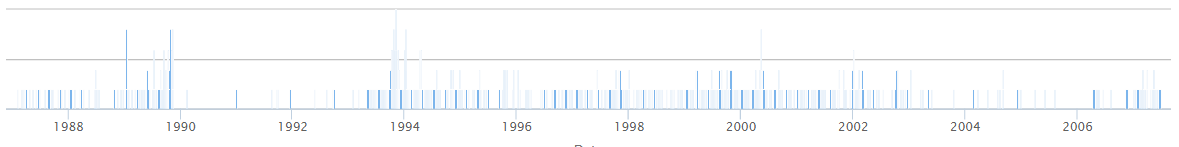
\includegraphics[width=\textwidth]{images/rg_timeline.png}
    \caption{Temporal distribution of top 1000 documents for \texttt{Rudolph Giuliani}}
    \label{fig:temporal_rg}
\end{figure}

\begin{figure}[!h]
\centering
 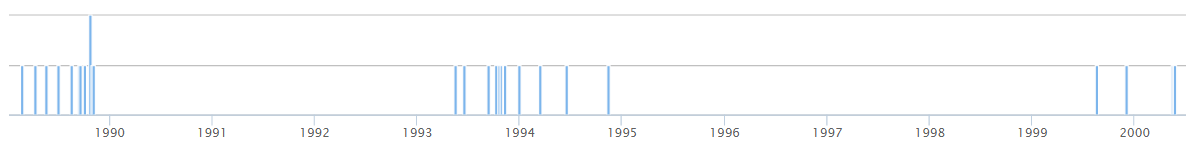
\includegraphics[width=\textwidth]{images/rg_timeline_pm230.png}
    \caption{Temporal distribution of top 1000 documents for \texttt{Rudolph Giuliani} after diversification using \textbf{T-PM2}}
    \label{fig:temporal_rg}
\end{figure}

\begin{figure}[!h]
\centering
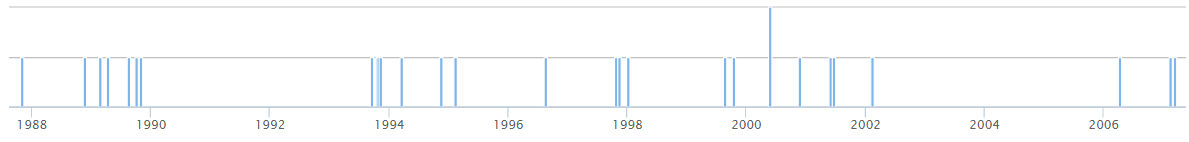
\includegraphics[width=\textwidth]{images/rg_timeline_iasel30.png}
    \caption{Temporal distribution of top 1000 documents for \texttt{Rudolph Giuliani} after diversification using \textbf{T-IASEL}}
    \label{fig:temporal_rg}
\end{figure}

\begin{figure}[!h]
\centering
 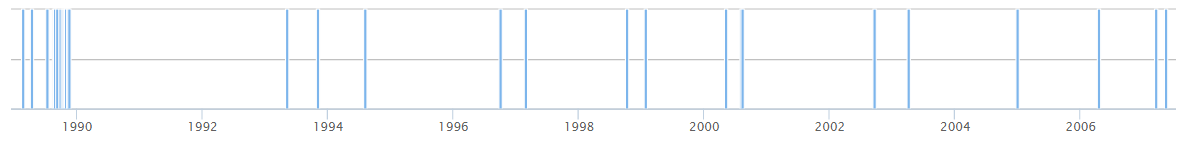
\includegraphics[width=\textwidth]{images/rg_timeline_mdiv30.png}
    \caption{Temporal distribution of top 1000 documents for \texttt{Rudolph Giuliani} after diversification using \textbf{T-MDIV}}
    \label{fig:temporal_rg}
\end{figure}

\begin{figure}[!h]
\centering
 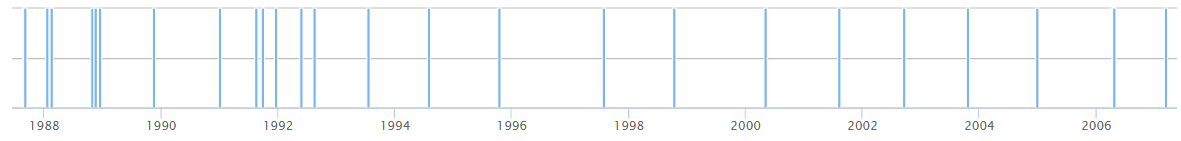
\includegraphics[width=\textwidth]{images/rg_timeline_lmtd30.png}
    \caption{Temporal distribution of top 1000 documents for \texttt{Rudolph Giuliani}after diversification using \textbf{Only Time}}
    \label{fig:temporal_rg}
\end{figure}

\begin{figure}[!h]
\centering
 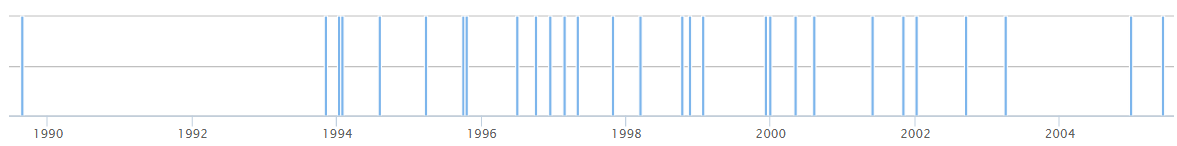
\includegraphics[width=\textwidth]{images/rg_timeline_histdiv30.png}
    \caption{Temporal distribution of top 1000 documents for \texttt{Rudolph Giuliani}after diversification using \textbf{HistDiv}}
    \label{fig:temporal_rg}
\end{figure}


% subsection qualitative_results (end)
% qualitative results


% \textbf{intro} In this section we discuss the outcome of our experiments. We present the results at k=10 for the measures TIA-NDCG, TIA-ERR,  SBR, TIA-PRECISION and TA-MAP in table 1. It is clear that HistDiv outperforms its competitors in all measures except TIA-Precision where the diversity by propotionality (PM2) approach is slightly better. It is also clear that the algorithms that take time into account explicitly perform better than just aspect based diversification with the exception being PM2 again. MDIV which takes both dimensions into account like HistDiv also performs reasonably well.

% \textbf{good} First lets take a look at the user centric methods like NDCG and ERR. The time awareness added to these measures indicates the extent to which a user has to scroll down the list in order to find a relevant result to his intent from the corresponding important time period. ERR helps guage the extent to which the average user has to scroll through this list in order to find a relevant result whereas NDCG is used to measure the cummulative information gain of a list. The gain for each document in the list is discounted depending on its rank due to the assumption that the user is less likely to keep scrolling down the list. Thus documents from lower ranks contribute little to the cummulative gain of a ranked list.  HistDiv outperforms its competitors in both user centric measures due to its unique calculation of time and aspect utility. The first document in a ranked list generated by HistDiv is from the most important time window with the most important aspects or vice versa depending on the tuning parameters. The aspects of the document are then discounted only within a certain time interval defined by the decay function. This allows HistDiv to reselect the same aspect but from a different time window thereby increasing its temporal awareness. Similarly if the document only covers a small portion of important aspects in a time window, HistDiv can revisit the time window to find a relevant document with diverse aspects which could increase the probability of covering a different subtopic.

% \textbf{good} HistDiv is significantly better at SBR when compared to its competitors. Its also clear that Temporal IA Select, MDIV and LD+T+D are superior to their original non-temporal counterparts in all measures. IA-SELECT only considers aspects for diversification and hence performs poorly in our modified SBR. An interesting outcome of these experiments is the performance of PM2 and Temporal PM2. Unlike Temporal IA-SELECT, Temporal PM2 performs worse in almost every measure even when compared to its non temporal counterpart. This phenomenon can be attributed to PM2's approach of not penalizing the over representation of an aspect. Most of the documents for Rudolph Giuliani refer to his election campaigns which PM2 tries to represent proptionaly in the result set and hence it performs quite poorly at subtopic recall . Non Temporal PM2 by virtue of being time averse actually does better because it represents the election campaigns from a wider time range. The linearized aspects for Temporal PM2 on the other hand enforce the representation of the campaign from the most important year only, thus leading to a smaller temporal spread. It must be noted that PM2 by virtue doesnot conform to the traditional assumption of diversity that one document is enough for one aspect. They introduce their own metric CPR to measure propotionality of the result list. In our experiments, we found that they are better than all other competitors for their metric even for historical query intents. Our closest competitor in subtopic recall is OnlyTime. Even though this algorithm is only concered with time based diversity, it performs well due to the nature of subtopics in historical search. A subtopic for a historical intent can either be an important event or a type of event that occurs across a time period in history. If the time spans of subtopics are disjoint then purely by introducing a temporal spread, diversity can be acheived. 

% \textbf{TIA-SBR} From SBR, it is evident that certain algorithms generate a better temporal spread than others. However, at times it is deterimental to just introduce a spread over time if the time windows covered are not important. Unlike SBR, TIA-SBR considers the weight of each time window when calculating recall in order to reward algorithms that pick documents that are diverse and from important time windows.The modeling of time windows as bursts explicity helps maintain HistDiv's supeririority in not only SBR but TIA-SBR as well. From table x, we can see that HistDiv is better than all other algorithms even at varying depths when it comes to TIA-SBR. In the same table we also show the number of queries from the 30 query workload for which each algorithm is better than LM. HistDiv's modeling of aspect importance decaying over time helps it choose the most relevant aspects for a given time period. These aspects can be covered again thanks to the temporal utility function $\delta_a$, which discounts aspect utility only within a certain time frame. HistDiv can also handle the fact that a single important time window can be quite diverse in itself so even though it may not have a greater temporal spread than OnlyTime, it will have a better chance at maximizing subtopic recall. MDIV is the only other algorithm that also accounts for 2 dimensions like HistDiv explicitly. MDIV's rank based approach to computing utility does not hold it in good stead though. The generic approach to discounting neither accurately models the temporal diversity of an aspect nor the aspect diversity of a single time window. The discounting based on the rank of a document in a given dimension is averse to the influence of the other dimension. HistDiv on the other hand considers the influence of time in the aspect dimension and vice versa.

% \textbf{bad} All is not rosy though if you are HistDiv. HistDiv's eagerness to diversify both dimensions sees it take a minor hit when it comes to TIA-Precision. This can be atrributed to the nature of some topics which are bound very closely to a small time window with very little aspect diversity, like \emph{reunification of germany}. For the given tuned parameters, if HistDiv covers enough important aspects in the important time windows it will start looking for documents with important aspects in other less relevant windows. Algorithms like PM2 which lock on to heavy time windows in order to proptionally diversify them do well in precision due to the sheer dominant weight of the time window. These methods suffer at recall because they serve as many relevant documents as they can for the heavy time window. So even though HistDiv has good recall for a topic it will suffer slightly when it comes to precision purely because of these very heavy bursts and HistDiv's calibration towards covering more subtopics rather proptionally representing time windows. 

% (Dont think this is needed) There are certain types of topics for which HistDiv is outperformed by its competitors. Consider the topic Summer Olympics Doping Scandals. The user's intent is to know the history of all doping scandals at the summer olympics between 1987 and 2007. The subtopics of this topic as per our test collection are: 

% \begin{enumerate}

%   \item 1988 Seoul - doping mostly in wrestling and judo
%   \item 1992 Barcelona - mostly athletics related cases
%   \item 1996 Atlanta - very few cases. only 2 in athletics.
%   \item 2000 Sydney - quite a few in athletics and weight lifting. Marion Jones was the most popular one.
%   \item 2004 Athens- Massive increase in doping compared to previous years
%   \item Measures taken by the IOC to combat doping
% \end{enumerate}

% From the subtopics there is no clear important time window for this topic and it seems like a straightforward temporal diversity case. Also we consider equal importance of subtopics like traditional diversity methods. However since the underlying corpus is the New York Times, the majority of doping stories emanate from the Marion Jones case from 2000. Reports in the following years then continue to follow Jones and talk about her until the 2004 olympics. The 2004 olympics saw a sudden spike in doping cases as well leading to a large number of articles publised about doping in 2004. Thus the time awareness of metrics here hurts methods which actually try to introduce wide temporal spread to cover the other subtopics. Temporal PM2 due to its nature to proptionally represent aspects restricts the majority of top documents to the dominant time window. ASPTD on the other hand does not favour proptionality so it tends to start traveling outside the important time windows to look for diverse events once it has covered the important time periods and the most important aspects. Time awareness in the metrics here penalizes ASPTD unfairly. For topics with disproptionately heavy time windows, temporal PM2 does well. (this is the same reason we do badly in precision)


% Another case where ASPTD is not the best is for historical intents whose subtopics are broad disjoint categories like \emph{elections in the middle east}. Here the subtopics are divided based on region and no temporal aspect is present. As expected in such cases, IA-SELECT is the best performing algorithm. Since there are no major time windows the lack of a temporal dimension does not hurt the performance of the algorithm. From these observations we can conclude that HistDiv, without specific parameter tuning, is not particularly competitive to diversification problems of a purely temporal or non-temporal nature.


